% Behaviour of the stator voltage and the RMS-value of the stator
% flux as a function of speed in scalar control.
% Author: Paul Nong-Laolam <pnong-laolam@espec.com> Software Engineer 
% Date: Nov 13, 2024 
% Simulation side: https://latex.org/forum/viewtopic.php?t=1441
\documentclass{article}
\usepackage{amsmath} % Required for \varPsi below
\usepackage{tikz}
\begin{document}

\begin{center} 
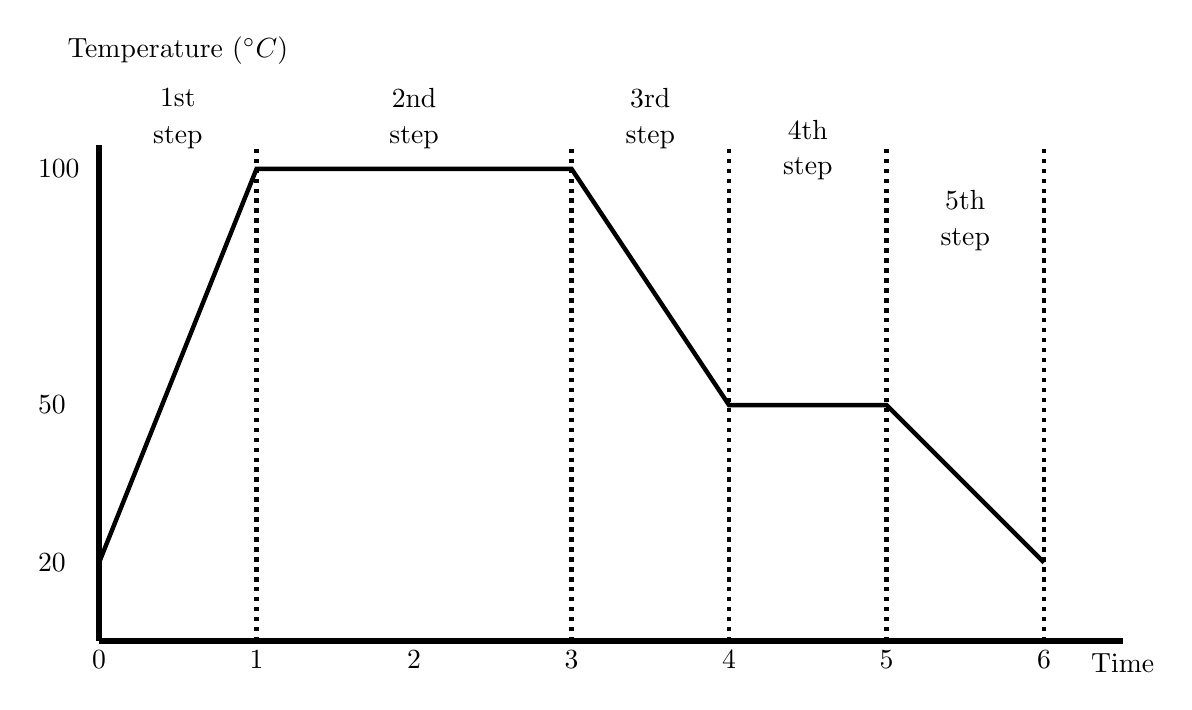
\begin{tikzpicture} [scale=2]

% horizontal axis
\draw [line width=0.8mm] (0,0) -- (6.5,0) node[anchor=north] {Time};

% labels
\draw	(0,0) node[anchor=north] {0}
		(1,0) node[anchor=north] {1}
		(2,0) node[anchor=north] {2}
		(3,0) node[anchor=north] {3}
		(4,0) node[anchor=north] {4}
		(5,0) node[anchor=north] {5}
		(6,0) node[anchor=north] {6};
		
% TEST on verticale axis
\draw	(-0.45,0.5) node[anchor=west] {20}
		(-0.45,1.5) node[anchor=west] {50}
		(-0.45,3) node[anchor=west] {100};
		
% ranges
\draw	%(1,3.5) node{{\scriptsize Constant flux}}
		%(3,2.25) node{{Constant Value Operation}};
		(0.5,3.75) node{{Temperature ($ ^{\circ} C$)}};

% vertical axis
\draw [line width=0.8mm] (0,0) -- (0,3.15) node[anchor=east] {};

% nominal speed
\draw [dotted, ultra thick] (1,0) -- (1,3.15)
      %[dotted, ultra thick] (2,0) -- (2,3.15)
      [dotted, ultra thick] (3,0) -- (3,3.15)
      [dotted, ultra thick] (4,0) -- (4,3.15)
      [dotted, ultra thick] (5,0) -- (5,3.15)
      [dotted, ultra thick] (6,0) -- (6,3.15);

% set labels on x-axis 
\draw [ultra thick] (0,0.5) -- (1,3) -- (3,3) -- (4,1.5) -- (5,1.5) -- (6,0.5);

% put labels on each time slice 
\draw [line width=1] (0.5,3.45) node {1st}; %label
\draw [line width=1] (0.5,3.20) node {step}; %label

\draw [line width=1] (2.0,3.45) node {2nd}; %label
\draw [line width=1] (2.0,3.20) node {step}; %label

\draw [line width=1] (3.5,3.45) node {3rd}; %label
\draw [line width=1] (3.5,3.20) node {step}; %label

\draw [line width=1] (4.5,3.25) node {4th}; %label
\draw [line width=1] (4.5,3.00) node {step}; %label

\draw [line width=1] (5.5,2.80) node {5th}; %label
\draw [line width=1] (5.5,2.55) node {step}; %label

%\draw [ultra thick] (0,0) -- (2,2) -- (6,2);
%\draw [line width=3]  (-0.45,2) node {30 $ ^{\circ} C$}; %label
%\draw [line width=1] (0,-0.4) node {Start of}; %label
%\draw [line width=1] (0,-0.6) node {constant value}; %label
%\draw [line width=1] (0,-0.8) node {operation}; %label
%\draw [line width=2] (6,-0.4) node {End of}; %label
%\draw [line width=2] (6,-0.6) node {constant value}; %label
%\draw [line width=2] (6,-0.8) node {operation}; %label
%\draw (1,1.5) node {$U_s$}; %label

% Psis
%\draw[thick,dashed] (0,3) -- (2,3) parabola[bend at end] (6,1);
%\draw (2.5,3) node {$\varPsi_s$}; %label

\end{tikzpicture}
\end{center}
\end{document}
